\documentclass{article}
\usepackage{amsmath,amsfonts,amsthm,amssymb}
\usepackage{fullpage,fancyhdr}
\usepackage[pdftex]{graphicx}
\usepackage[usenames,dvipsnames]{color}
\usepackage{listings}
\usepackage{courier}
\usepackage{ifthen}
\usepackage{setspace}
\usepackage{lastpage}
\usepackage{extramarks}
\usepackage{chngpage}
\usepackage{soul}
\usepackage{graphicx,float,wrapfig}
\usepackage{epstopdf}
\usepackage{geometry}
\usepackage{pdfcolmk}
\usepackage{hyperref}
\usepackage{epsfig}
\DeclareGraphicsRule{.tif}{png}{.png}{`convert #1 `dirname #1`/`basename #1 .tif`.png}

\definecolor{lightgray}{gray}{0.5}
\definecolor{darkgray}{gray}{0.3}
\definecolor{MyDarkGreen}{rgb}{0.0,0.4,0.0}

\topmargin=-0.45in      %
\evensidemargin=0in     %
\oddsidemargin=0in      %
\textwidth=6.5in        %
\textheight=9.0in       %
\headsep=0.25in         %

\pagestyle{fancyplain}
 
\fancyhf{}
 
\lhead{\fancyplain{}{Michael Carroll}}
\chead{\fancyplain{}{ELEC6230 - Parallel Processing}}
\rhead{\fancyplain{}{\today}}
\rfoot{\fancyplain{}{\thepage\ of \pageref{LastPage}}}

\sloppy
\setlength{\parindent}{0pt}

\lstloadlanguages{C++}
\lstset{
language=C++,
frame=single,
basicstyle=\ttfamily,
keywordstyle=[1]\color{Blue}\bf,
keywordstyle=[2]\color{Purple},
keywordstyle=[3]\color{Blue}\underbar,
identifierstyle=,
numbers=left,
numberstyle=\tiny\color{Blue},
stepnumber=5,
morekeywords={printf,atoi,omp,parallel,shared,schedule,reduction},
morekeywords=[2]{gettimeofday,matrixSize,omp_get_wtime,omp_set_num_threads}
}

% Alter some LaTeX defaults for better treatment of figures:
% See p.105 of "TeX Unbound" for suggested values.
% See pp. 199-200 of Lamport's "LaTeX" book for details.
%   General parameters, for ALL pages:
\renewcommand{\topfraction}{0.9}	% max fraction of floats at top
\renewcommand{\bottomfraction}{0.8}	% max fraction of floats at bottom
%   Parameters for TEXT pages (not float pages):
\setcounter{topnumber}{2}
\setcounter{bottomnumber}{2}
\setcounter{totalnumber}{4}     % 2 may work better
\setcounter{dbltopnumber}{2}    % for 2-column pages
\renewcommand{\dbltopfraction}{0.9}	% fit big float above 2-col. text
\renewcommand{\textfraction}{0.07}	% allow minimal text w. figs
%   Parameters for FLOAT pages (not text pages):
\renewcommand{\floatpagefraction}{0.7}	% require fuller float pages
% N.B.: floatpagefraction MUST be less than topfraction !!
\renewcommand{\dblfloatpagefraction}{0.7}	% require fuller float pages

% remember to use [htp] or [htpb] for placement

\title{ELEC6230 Final Project\\
{\large \begin{par}
Results of Parallel Processing Final Project
\end{par} \vspace{1em}
}}
\author{Michael J. Carroll}

\begin{document}
\maketitle

\section*{Introduction}
\begin{par}
The purpose of this project was to write an iterative convolution algorithm in two different parallel processing environments and benchmark/compare the results to that of a sequential algorithm.  To accomplish this, I utilized the Alabama Super Computer that we were given access to for the class.  All benchmark results were executed on the Altix cluster of the ASC.  I choose to implement my algorithms in MPI and OpenMP, as well as the sequential C++ program.
\end{par}

\section*{Predicted Results}
\subsection*{Sequential Programming}
\begin{par}
Before setting out to program, I first calculated what the approximate speedup and efficiency for each implementation should be.  Defining W as the width of the convolution window and N as the width of the image, inside of the actual convolution summation, there are $W^2$ additions and $W^2$ multiplications.  These are performed a total of $N^2$ times.  This entire convolution would then be performed twice. This leads to a total time complexity of $O(2 \times N^2 \times (W^2 \times 2))$ for a sequential implementation.  The overhead for sequential programming is negligible.
\end{par}

\subsection*{OpenMP Programming}
\begin{par}
From the sequential results, it is possible to expand to determine approximately what the time complexity of a parallel implementation will be.  To begin with, I looked at the OpenMP implementation.  OpenMP will directly divide the amount of processing to be done over the number of processing elements available.  In my case, I was to test PE = 2,3,4,5,6.  This would lead to a linear speedup and a peak efficiency.  Assuming perfect load balancing, the time complexity of the OpenMP algorithm should be exactly the same as that of the sequential, but divided by the number of processing elements.   The overhead will make the solution slower, as OpenMP will then have to synchronize the entire contents of memory over the rest of the processing elements.
\end{par}

\subsection*{MPI Programming}
\begin{par}
The MPI results should be similar in time complexity to the OpenMP results, but they should have less communication overhead than that of the OpenMP results.  The reason for this is that OpenMP is syncing the entire memory (2160x2160) between the two iterations of the convolution.  With the MPI algorithm, it is theoretically possible to make significantly less transfers between the two iterations.  Since the window size is 11, then only 5 rows from the top and bottom of each PEs memory will have to be transferred.  This makes the worse case transfer $(2 \times 5 \times 2160 \times \# of PEs)$ for the time between iterations.  While the computational time complexity should be about the same as OpenMP, the reduced transfer overhead of MPI should have increased speedups.  A summary of my findings is in Table~\ref{tbl:comparison}.
\end{par}

\begin{table}
\begin{tabular}[tbph]{lll }
Programming Type & Computational Time Complexity & Overhead \\
Sequential Programming & $4N^{2}W^{2}$ & Negligible \\
OpenMP Programming & $\frac{4N^{2}W^{2}}{P}$ & $N^{2}$ Per Iteration \\
MPI Programming & $\frac{4N^{2}W^{2}}{P}$ & $2  \lfloor W/2 \rfloor NP$\\
\end{tabular}
\caption{Comparison of Time Complexity of programming types}
\label{tbl:comparison}
\end{table}

\section*{Actual Results}
\begin{par}
Once I predicted what my performance speedups would be, I began to write the actual code.  I first implemented the sequential program, available in Appendix A.  From the original image in Figure~\ref{fig:inpimg}, I was able to produce the output in Figure~\ref{fig:seqimg}.  Part of the project requirements was to not use any of the Intel C Compiler's built-in optimizations or speedups, so I left those options out during the compiling process.  I found the sequential program to operate at 8.45 seconds, on average, for the the two iterations of the convolution. \\
\\
From the sequential results, I could then get the parallel results.  The interface that I programmed for first was OpenMP.  The image output of the OpenMP program is included in Figure~\ref{fig:ompimg}\\
\\
Finally, I was able to program for the MPI programming environment.  The MPI environment posed several more significant hurdles over the OpenMP programming.  The main problem was handling the message passing between iterations of the convolution. The math to pass the bottom and top rows to neighboring cells became overwhelming quickly and was nearly impossible to debug on the system.  The output that I managed to produce for the MPI algorithm was still noisier than that of the sequential algorithm and the OpenMP algorithm.  This image is included in Figure~\ref{fig:mpiimg}.  The noise may not be visible in this document, but it does exist.  I believe that this additional noise may be due to the fact that my algorithm was somehow incomplete and did not completely cover the image in the way that it was supposed to.
\end{par}

\begin{par}
The final results of all of my runs are included in Table~\ref{tbl:spdeff}.  The OpenMP algorithm is by far the best performance and efficiency-wise, counter to my theoretical results.  The MPI algorithm was much slower than even the sequential performance time, which leads me to believe that there may be more wrong with the algorithm, rather than the technology behind it.  The speedup and efficiency plots are included in Figure~\ref{fig:spd} and Figure~\ref{fig:eff}, respectively.
\end{par}

\begin{table}
\centering
\begin{tabular}[htbp]{| l | r | r | r | r | r | r |}
\hline
Number of Processing Elements  & 1 & 2 & 3 & 4 & 5 & 6 \\
\hline
\textbf{Sequential Operation} & 8.5 & & & & & \\
\hline
\textbf{OpenMP} & 8.58 & 4.30 & 2.9 & 2.17 & 1.74 & 1.52 \\
Speedup & 1.00 & 1.99 & 2.95 & 3.95 & 4.93 & 5.64 \\
Efficiency & 100 & 99.8 & 98.6 & 98.9 & 98.6 & 94.1 \\
\hline
\textbf{MPI}  & 82.5 & 55.4 & 37.8 & 28.7 & 22.9 & 19.3 \\
Speedup & 1.00 & 1.49 & 2.18 & 2.87 & 3.60 & 4.27 \\
Efficiency & 100 & 74.5 & 72.8 & 71.9 & 72.0 & 71.2 \\
\hline
\end{tabular}
\caption{Comparison of Speedup and Efficiency}
\label{tbl:spdeff}
\end{table}

\begin{figure}[htbp]
\centering
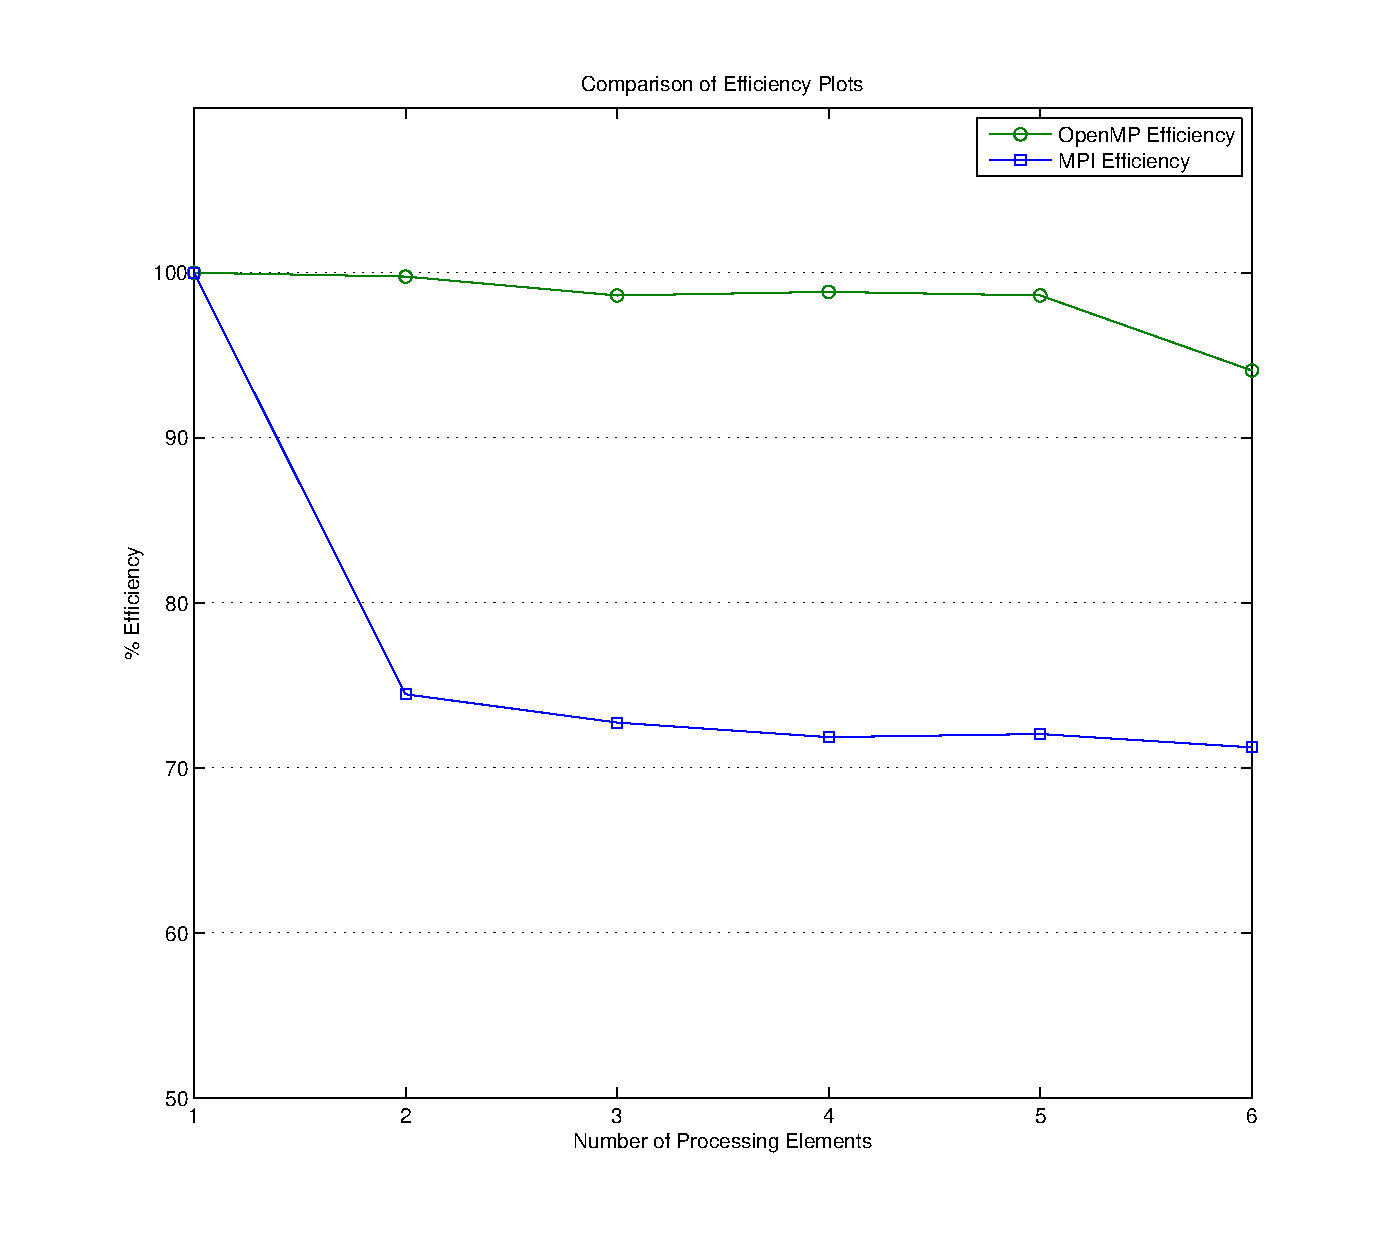
\includegraphics[width=0.6\linewidth]{efficiency.eps}
\caption{Efficiency Comparison}
\label{fig:eff}
\end{figure}

\begin{figure}[htbp]
\centering
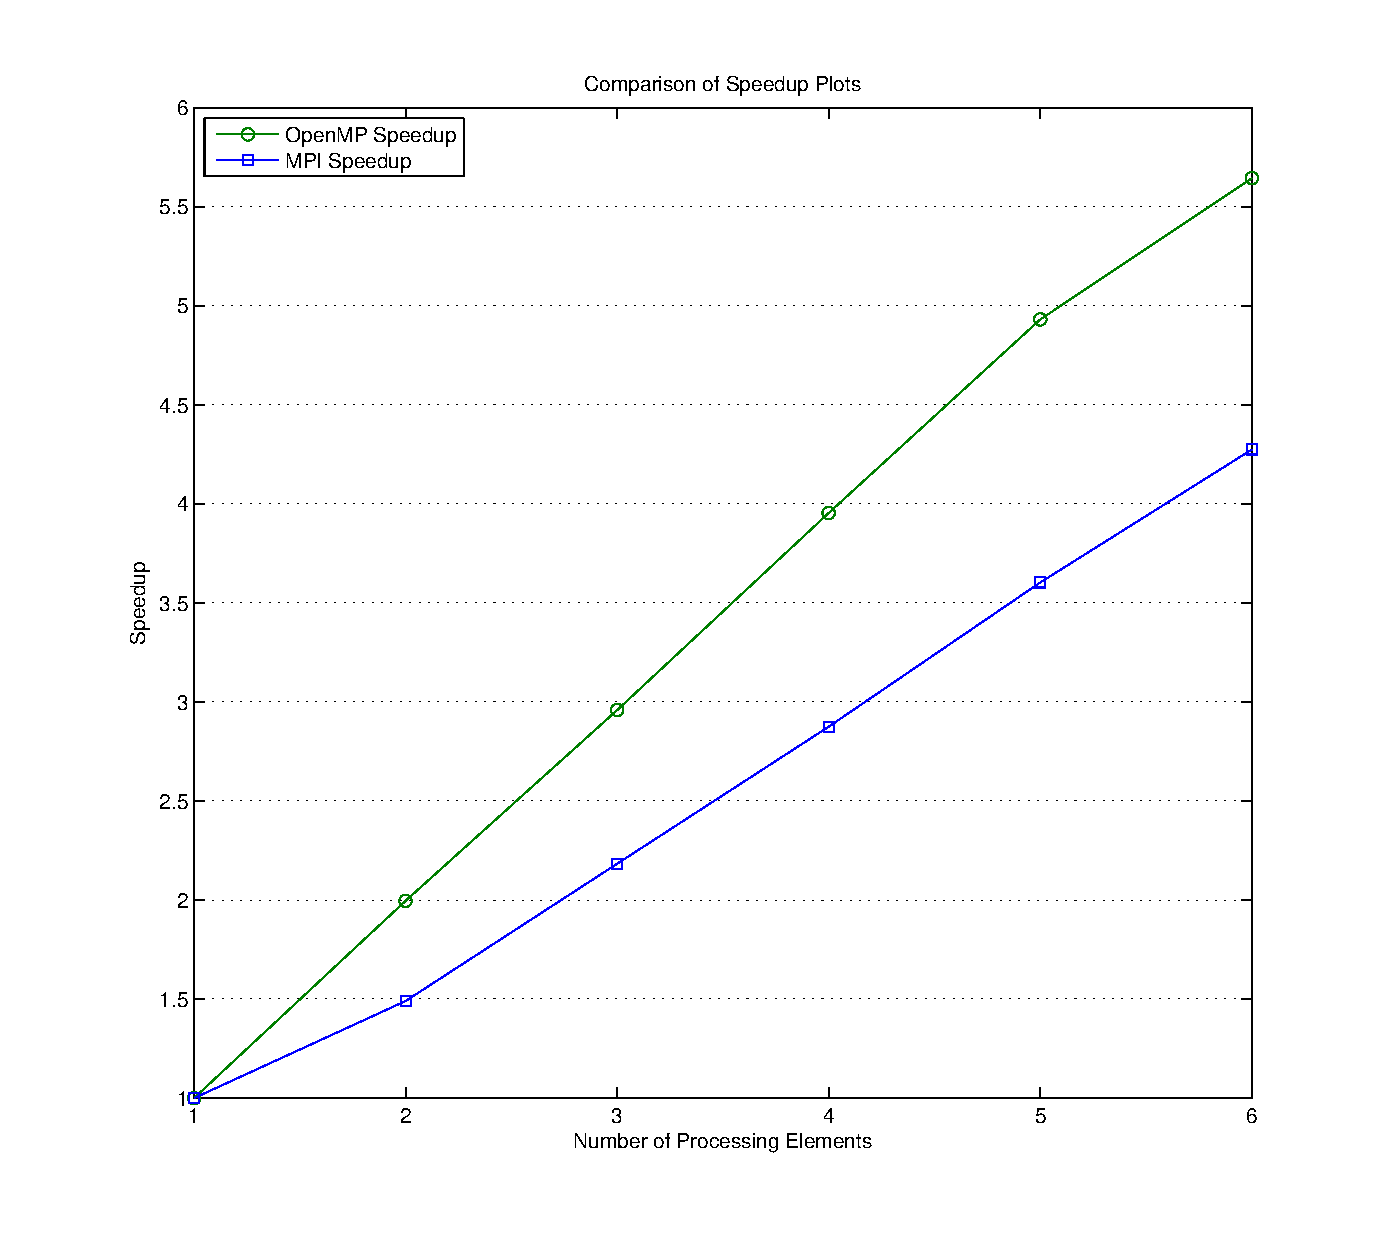
\includegraphics[width=0.6\linewidth]{speedup.eps}
\caption{Speedup Comparison}
\label{fig:spd}
\end{figure}

\section*{Comparison of theoretical and actual performance}
\begin{par}
While my mathematics showed that the MPI programming interface should be much faster in theory, it ended up being that the OpenMP interface was the fastest.  This is probably partially due to the fact that the MPI code was very difficult to debug.\\
\\
The OpenMP interface had the same time for one processing element as the sequential operation, and had a near-linear speedup.  It is faster than the sequential operation by a factor of $1/PEs$.  The more processing elements added, the faster that the convolution problem was solved.  This would probably also hold true with more and more processing elements as well as more convolution iterations.\\
\\
The MPI was an order of magnitude slower than the sequential operation, making it difficult to compare to the other two algorithms.  While it's speedup and efficiency were relatively constant, the fact that it was so much slower, even with 1 processing element makes it a difficult algorithm to consider.
\end{par}

\section*{Conclusions}
\begin{par}
Through this exercise, I learned a great deal more about both the OpenMP and MPI programming interfaces.  In future endeavors, I am much more likely to choose the OpenMP platform due to ease of use and incredible performance on the project.  While I did not consider CUDA programming in the scope of this project, I am sure that it too would be significantly faster than the sequential operation.\\
\\
The OpenMP interface seems to be much more user-friendly and better documented than the MPI code interface.  While MPI is a large standard that is used in many projects, it is hard to find examples of other people solving problems with it.  The lack of resources available for MPI vs those available for OpenMP (and CUDA) make OpenMP the better platform in comparison.
\end{par}

\begin{figure}[htbp]
\begin{minipage}[b]{0.5\linewidth}
\centering
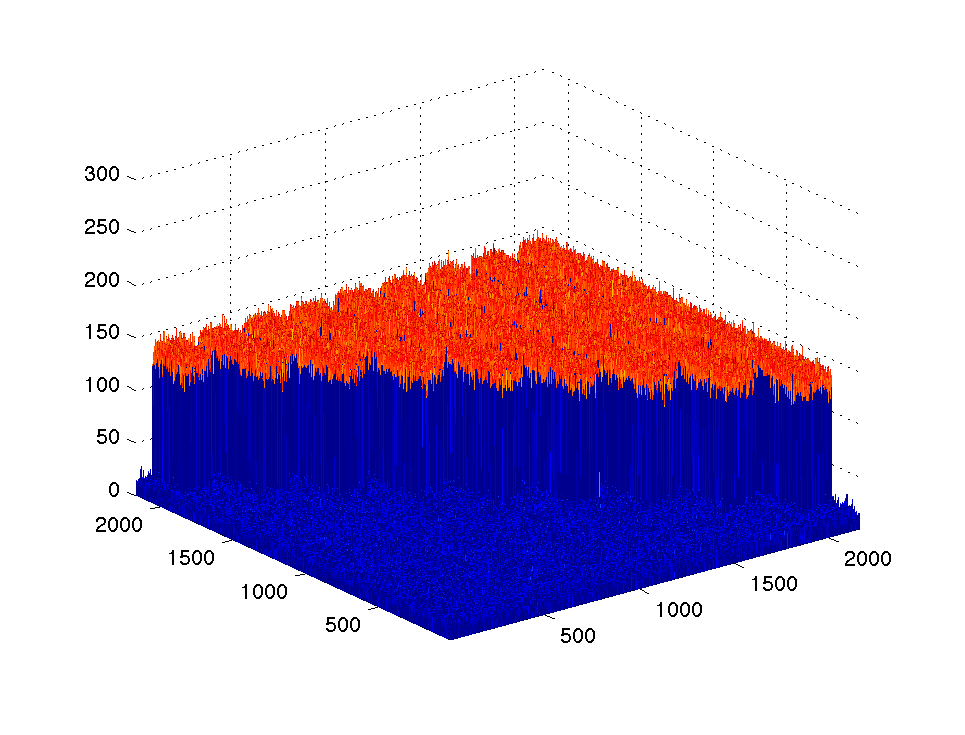
\includegraphics[width=\linewidth]{Original-image.eps}
\caption{Input Image}
\label{fig:inpimg}
\end{minipage}
\hspace{0.5cm}
\begin{minipage}[b]{0.5\linewidth}
\centering
\includegraphics[width=\linewidth]{sequential-image.eps}
\caption{Image Results from Sequential}
\label{fig:seqimg}
\end{minipage}
\end{figure}

\begin{figure}[htbp]
\begin{minipage}[b]{0.5\linewidth}
\centering
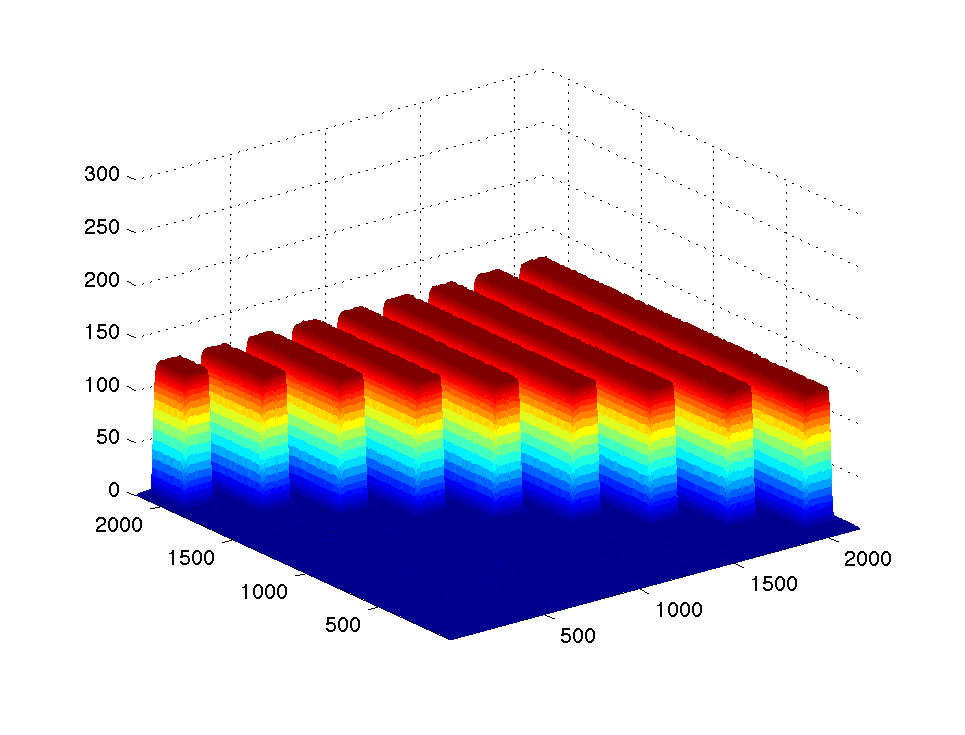
\includegraphics[width=\linewidth]{openmp-image.eps}
\caption{Image Results from OpenMP}
\label{fig:ompimg}
\end{minipage}
\hspace{0.5cm}
\begin{minipage}[b]{0.5\linewidth}
\centering
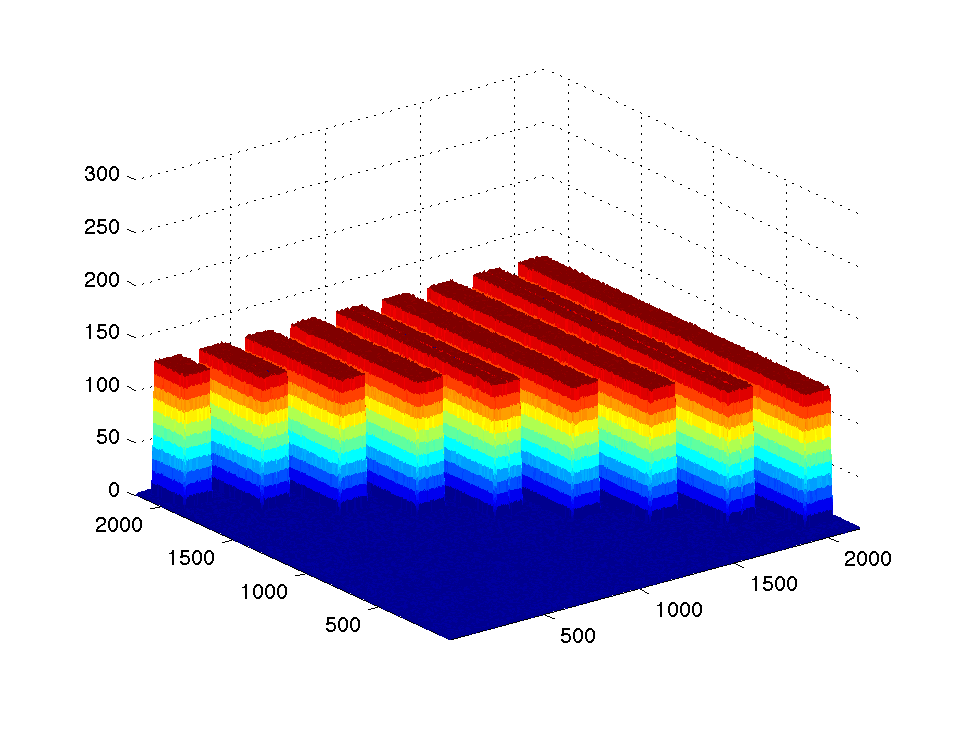
\includegraphics[width=\linewidth]{mpi-image.eps}
\caption{Image Results from MPI}
\label{fig:mpiimg}
\end{minipage}
\end{figure}


\newpage
\section*{Appendix A - Sequential Implementation}
\lstinputlisting{../sequential.cpp}

\newpage
\section*{Appendix B - OpenMP Parallel Implementation}
\lstinputlisting{../parallel-omp.cpp}

\newpage
\section*{Appendix C - MPI Parallel Implementation}
\lstinputlisting{../parallel-mpi.cpp}

\end{document}